\section{Tổng quan nghiên cứu} % Section 2

\subsection{Tình hình nghiên cứu hiện tại} % 2.1

Nhận diện biểu cảm khuôn mặt (Facial Expression Recognition - FER) là một nhánh quan trọng trong lĩnh vực trí tuệ nhân tạo (AI) và thị giác máy tính. Trong những năm gần đây, nhờ sự phát triển của học sâu (Deep Learning), đặc biệt là mạng nơ-ron tích chập (Convolutional Neural Networks - CNN), hiệu suất của các hệ thống FER đã được cải thiện đáng kể. Các mô hình như VGGNet, ResNet, Inception, và gần đây là EfficientNet và Vision Transformer đã đạt độ chính xác cao trên nhiều tập dữ liệu chuẩn như FER-2013, CK+, JAFFE, và AffectNet.

Tuy nhiên, đa số các nghiên cứu tập trung vào điều kiện ánh sáng chuẩn, trong khi điều kiện ánh sáng yếu vẫn còn là một thách thức lớn. Trong môi trường ánh sáng yếu, đặc trưng khuôn mặt bị mất thông tin, độ tương phản thấp, dẫn đến độ chính xác giảm đáng kể. Để giải quyết vấn đề này, một số nghiên cứu gần đây đã đề xuất sử dụng các kỹ thuật như tăng cường dữ liệu ánh sáng yếu (Low-Light Data Augmentation), cải thiện độ sáng bằng GAN (EnlightenGAN, RetinexNet), hoặc sử dụng bộ tăng cường ánh sáng học sâu. Mặc dù các phương pháp này cho kết quả tốt, chúng thường đòi hỏi mô hình phức tạp và tài nguyên tính toán lớn.

Bên cạnh đó, xu hướng nghiên cứu gần đây cũng tập trung vào các mô hình nhẹ (Lightweight CNNs) như MobileNet, ShuffleNet, hoặc SqueezeNet nhằm đáp ứng yêu cầu triển khai thực tế trên thiết bị di động hoặc hệ thống nhúng. Một số công trình kết hợp mô hình nhẹ với chiến lược huấn luyện thông minh hoặc tăng cường dữ liệu thích ứng để cải thiện hiệu quả trong điều kiện môi trường thay đổi, bao gồm ánh sáng yếu.

\subsection{Hướng tiếp cận của đề tài} % 2.2

Đề tài tập trung vào việc giải quyết bài toán nhận diện biểu cảm khuôn mặt trong điều kiện ánh sáng yếu thông qua hai hướng tiếp cận chính:

\begin{figure}[H]
    \centering
    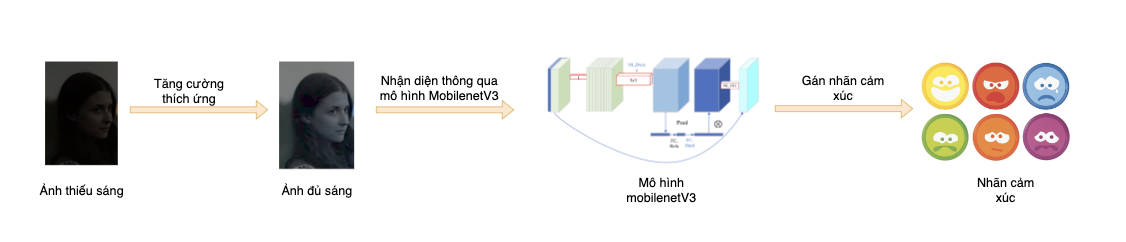
\includegraphics[width=12cm]{./img/phuong_phap_tiep_can.png} \\[0.5cm]
    \caption{Sơ đồ tổng quan quá trình nhận diện biểu cảm khuôn mặt trong điều kiện ánh sáng yếu sử dụng mô hình MobileNetV3 kết hợp tăng cường dữ liệu thích ứng.}
    \label{fig:phuong_phap_tiep_can}
\end{figure}

\begin{itemize}
    \item \textbf{Sử dụng mô hình CNN nhẹ:} MobileNetV3 được lựa chọn làm kiến trúc mạng nơ-ron nền tảng vì có dung lượng nhỏ, tốc độ suy luận nhanh và phù hợp triển khai trên thiết bị giới hạn tài nguyên. Điều này giúp đảm bảo tính khả thi trong các ứng dụng thực tế như camera an ninh, robot xã hội, hay thiết bị đeo thông minh.
    
    \item \textbf{Tăng cường dữ liệu thích ứng:} Khác với các phương pháp tăng cường dữ liệu cố định, đề tài đề xuất kỹ thuật tăng cường dựa trên mức độ sáng của từng ảnh đầu vào. Các phép biến đổi như điều chỉnh gamma, contrast stretching sẽ được áp dụng linh hoạt để mô phỏng đa dạng điều kiện ánh sáng yếu, giúp mô hình học được các đặc trưng biểu cảm một cách ổn định hơn.
\end{itemize}

Hướng tiếp cận này vừa đảm bảo hiệu quả nhận diện trong điều kiện ánh sáng khó khăn, vừa phù hợp với yêu cầu triển khai thực tế. Đề tài không chỉ có ý nghĩa trong việc nâng cao chất lượng hệ thống FER, mà còn mở ra khả năng mở rộng cho các bài toán thị giác máy tính khác trong môi trường bất lợi.

\subsection*{Câu hỏi nghiên cứu} % 2.3

Từ thực trạng và hướng tiếp cận đã trình bày, đề tài tập trung trả lời các câu hỏi nghiên cứu chính sau:

\begin{itemize}
    \item Việc áp dụng kỹ thuật tăng cường dữ liệu thích ứng theo mức độ sáng có giúp cải thiện hiệu suất nhận diện biểu cảm khuôn mặt trong điều kiện ánh sáng yếu hay không?
    
    \item Mô hình CNN nhẹ (MobileNetV3) khi kết hợp với dữ liệu đã được tăng cường thích ứng có thể đạt độ chính xác trên 70\% và đảm bảo tốc độ xử lý đủ nhanh để triển khai thực tế trên thiết bị tài nguyên thấp hay không?
\end{itemize}